\begin{problem}{TV 방송}
	{}{Output Only}
	{}{}{}
	
	이번에 JOI 왕국에서는 TV 방송을 시작하기로 했다. JOI 왕국에는 $N$ 채의 집이 있다. 이 집 모두가 TV를 볼 수 있도록 기지국을 설치하고 싶다.
	
	이번에 JOI 왕국의 왕은 $K$ 개의 전파탑을 설치하기로 했다. $i$ 번째 전파탑을 $(X_i, Y_i)$에 설치하고 출력 레벨을 $E_i$로 설정하면, $(X_i, Y_i)$부터 거리가 $\sqrt{E_i}$ 이하인 집에 TV 방송을 볼 수 있게 된다(두 점 $(a, b)$ 와 $(c, d)$ 사이의 거리는 $\sqrt{(a-c)^2 + (b-d)^2}$으로 주어진다). 단, 전파탑의 출력 레벨을 $E_i$로 설정하면, $E_i$의 에너지를 소비한다. 모든 집에서 TV 방송을 볼 수 있게 하면서, 가능한 한 $K$ 개 전파탑에서 사용하는 에너지 소비의 총합(이하, 소비 에너지)을 최대한 줄이고 싶다. 전파탑은 집이 있는 곳에 세울 수도 있으며, 같은 위치에 두 개를 설치해도 된다.
	
	JOI 왕국에 있는 집의 좌표가 주어졌을 때, 모든 집에서 TV 방송을 볼 수 있도록 전파탑을 세우는 장소와 출력 레벨을 정하고 싶다.
	
	JOI 왕국에 있는 집의 위치와 $K$가 주어질 때, 전파탑을 세우는 장소와 출력 레벨을 출력하여라. 소비 에너지가 적을수록 고득점이 된다.
	
	\Constraints
	
	\begin{tabular}{ll}
		$1 \le N \le 500$ & JOI 왕국에 있는 집의 수 \\
		$1 \le K \le 30$ & 설치할 전파탑의 수 \\
		$0 \le A_i, B_i \le 1\ 000\ 000$ & 집의 좌표
	\end{tabular}
	
	\InputFile
	
	다음 정보가 입력 파일로 주어진다.
	
	\begin{itemize}
		\item 첫째 줄에는 정수 $N$, $K$가 공백으로 구분되어 주어지며, JOI 왕국에 있는 집의 수가 $N$, 설치할 전파탑의 수가 $K$라는 것을 의미한다.
		\item 다음 $N$개의 줄의 $i$번째 줄에는 정수 $A_i$, $B_i$가 공백으로 구분되어 주어지며, $i$ 번째 집의 좌표가 $(A_i, B_i)$라는 것을 의미한다.
	\end{itemize}

	같은 좌표에 두 개 이상의 집이 있는 경우는 없다고 생각해도 된다.
	
	\OutputFile
	
	출력의 $i$ 번째 줄 ($1 \le i \le K$) 에는 세 개의 정수 $X_i$, $Y_i$, $E_i$ ($0 \le X_i \le 1\ 000\ 000$, $0 \le Y_i \le 1\ 000\ 000$, $0 \le E_i \le 1\ 000\ 000\ 000\ 000 (=10^{12})$)를 공백으로 구분하여 출력한다.

	\Scoring
	
	각 테스트케이스에 대해 득점은 다음과 같이 계산된다.
	
	참가자가 제출한 출력 중 소비 에너지의 최솟값을 $E_0$라고 하자. 제출한 출력이 문제의 조건을 만족하지 않을 경우, 점수는 0이다. 조건을 만족할 경우, 당신이 제출한 출력의 소비 에너지를 $E$라고 할 때,
	
	\begin{itemize}
		\item $\dfrac{E}{E_0}> 1.5$인 경우, 0
		\item $\dfrac{E}{E_0}\le 1.5$인 경우, $\left(4 \times {\left(1.5-\dfrac{E}{E_0}\right)}^2 \right) \times 20$을 소수점 첫째 자리에서 반올림한 값.
	\end{itemize}

	이 득점이 된다.
	
	\Examples
	
	\renewcommand{\InputFileName}{Sample Input}
	\renewcommand{\OutputFileName}{Sample Output}
	
	\begin{example}
		\exmp{
			10 3
			0 300000
			500000 800000
			700000 200000
			100000 500000
			400000 900000
			200000 1000000
			300000 500000
			300000 200000
			500000 100000
			1000000 0
		}{%
			200000 700000 160000000000
			300000 300000 90000000000
			750000 0 62500000000
		}%
	\end{example}

	이 입출력은 다음 그림에 대응된다. 각 원은 좌표 $(X_i, Y_i)$ 에서 거리 $\sqrt{E_i}$ 이하인 위치를 표시한다. 이 경우, 출력 에너지는 $160\ 000\ 000\ 000+90\ 000\ 000\ 000+ 62\ 500\ 000\ 000 = 312\ 500 \ 000 \ 000$ (3125억) 이다.	
	\begin{center}
	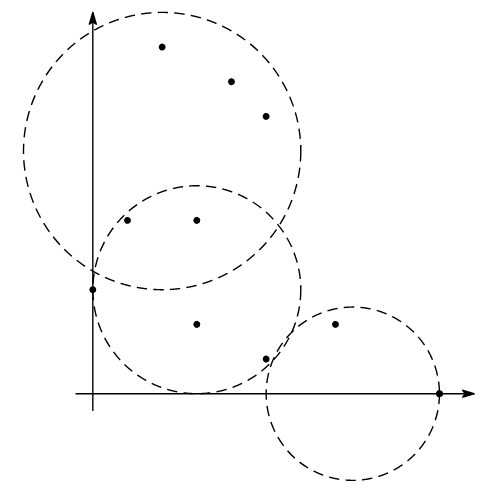
\includegraphics[width=0.5\linewidth]{img1.png}
	\end{center}	
\end{problem}

